% Exposición del paper «A Fast Wait-Free Solution to Read-Reclaim Races in Reference Counting» (Euro-Par 2024)
% Versión de 15 min. Expositores: David (parte 1), Jheremy (parte 2) y Diego (parte 3).
% Compilar: latexmk -pdf -interaction=nonstopmode -halt-on-error exposicion.tex
\documentclass[aspectratio=169,11pt]{beamer}
\usepackage[spanish,es-noshorthands,es-nodecimaldot,es-tabla]{babel}
\usepackage[T1]{fontenc}
\usepackage[sfdefault,lining]{FiraSans}
\usepackage[scale=0.86]{FiraMono}
\usepackage{booktabs,tabularx,array,graphicx,pifont,xcolor}
\usepackage{tikz}
\usetikzlibrary{arrows.meta,positioning,calc,babel}
\hypersetup{pdftitle={Exposición: A Fast Wait-Free Solution to Read-Reclaim Races in Reference Counting},pdfauthor={},pdfcreator={},pdfproducer={},pdfsubject={},pdfkeywords={}}

% ---------- paleta ----------
\definecolor{tinta}{HTML}{1B2430}
\definecolor{gris}{HTML}{5B6573}
\definecolor{acento}{HTML}{C8551F}   % el peso / talonario
\definecolor{hoja}{HTML}{1F5FA8}     % la hoja / contador
\definecolor{ok}{HTML}{1B7F3B}
\definecolor{mal}{HTML}{B3261E}
\definecolor{suave}{HTML}{EEF1F5}
\newcommand{\si}{\textcolor{ok}{\ding{51}}}
\newcommand{\no}{\textcolor{mal}{\ding{55}}}
\newcommand{\us}{\,\textmu s}
\newcommand{\clave}[1]{\textcolor{acento}{\textbf{#1}}}
\newcommand{\fuente}[1]{\par\vspace{2pt}{\scriptsize\color{gris}#1}}

% ---------- plantilla ----------
\setbeamertemplate{navigation symbols}{}
\setbeamercolor{normal text}{fg=tinta}
\setbeamercolor{structure}{fg=hoja}
\setbeamercolor{frametitle}{fg=tinta}
\setbeamerfont{frametitle}{size=\Large,series=\bfseries}
\setbeamertemplate{frametitle}{\vspace*{8pt}\insertframetitle\par\vspace{3pt}{\color{acento}\rule{1.6cm}{2.2pt}}\vspace*{-4pt}}
\setbeamertemplate{itemize item}{\textcolor{acento}{\small$\blacktriangleright$}}
\setbeamertemplate{itemize subitem}{\textcolor{gris}{--}}
\setbeamertemplate{enumerate item}{\textcolor{acento}{\bfseries\insertenumlabel.}}
\setbeamerfont{caption}{size=\scriptsize}
\newcommand{\elexpositor}{}
\newcommand{\expone}[1]{\renewcommand{\elexpositor}{#1}}
\setbeamertemplate{footline}{\leavevmode\hbox to\paperwidth{\hspace{10pt}\color{gris}\scriptsize%
  \ifx\elexpositor\empty\else Expone: \textbf{\textcolor{tinta}{\elexpositor}}\quad·\quad\fi
  de Wolff, Anderson, Keller y Seletskiy · Euro-Par 2024\hfill\insertframenumber\,/\,\inserttotalframenumber\hspace{10pt}}\vspace{6pt}}
\newcommand{\divisor}[4]{{\setbeamertemplate{footline}{}\begin{frame}[plain]
  \vfill{\color{acento}\large\bfseries Parte #1}\par\medskip{\fontsize{30}{34}\selectfont\bfseries #2}\par\bigskip
  {\large Expone: \textbf{#3}}\par\medskip{\color{gris}#4}\vfill\end{frame}}}
\setlength{\tabcolsep}{5pt}

\title{A Fast Wait-Free Solution to Read-Reclaim Races in Reference Counting}
\subtitle{Conteo de referencias concurrente: sin candados, sin esperas y sin memoria extra}
\date{}

\begin{document}

% =====================================================================
{\setbeamertemplate{footline}{}
\begin{frame}[plain]
  \vspace*{6mm}
  {\color{acento}\small\bfseries EXPOSICIÓN DE PAPER}\par\smallskip
  {\fontsize{24}{28}\selectfont\bfseries A Fast Wait-Free Solution to\\ Read-Reclaim Races in Reference Counting\par}
  \medskip
  {\large\color{gris}Conteo de referencias concurrente: sin candados, sin esperas y sin memoria extra\par}
  \vfill
  \begin{columns}[T]
    \column{0.50\textwidth}
    {\small\color{gris}Paper}\\
    Ivo Gabe de Wolff, Daniel Anderson, Gabriele K. Keller y Aleksei Seletskiy\\
    {\small Universidad de Utrecht · Carnegie Mellon University}\\
    {\small Euro-Par 2024 · LNCS 14803 · págs. 103–118 · doi 10.1007/978-3-031-69583-4\_8}
    \column{0.46\textwidth}
    {\small\color{gris}Expositores}\\[2pt]
    {\normalsize\bfseries David Tamo Turpo\par Jheremy Manuel Alvarez Astete\par Diego Quispe Candelario\par}
    \medskip{\small\color{gris}Artefactos}\\[2pt]
    {\small\href{https://claude.ai/artifact/YBS98Wz8SmSYWHca2YbHF6}{Artefacto 1} · \href{https://claude.ai/artifact/EQJd2aXZUYVX1Zio4DqFwH}{Artefacto 2} · \href{https://claude.ai/artifact/VVGviffH178bBZ6tGSAnKZ}{Artefacto 3}}
  \end{columns}
  \vspace*{4mm}
\end{frame}}

\expone{David}

\begin{frame}{El paper en una frase}
  \begin{block}{}
    \large ¿Cómo leer un puntero compartido a un objeto con conteo de referencias \textbf{mientras otro hilo lo cambia}, sin candados, sin que nadie espere y sin gastar memoria extra?
  \end{block}
  \bigskip
  \begin{itemize}
    \item Euro-Par 2024 (LNCS 14803), Utrecht y CMU; sello \emph{Artifact Evaluated}: el código es público y lo hemos usado.
    \item Mejora el \emph{split reference count} (Folly, GCC), que solo es \emph{lock-free}: la hace \textbf{\emph{wait-free}} y más sencilla de explicar.
  \end{itemize}
\end{frame}

\begin{frame}{Una analogía para toda la exposición}
  \renewcommand{\arraystretch}{1.1}\small
  \begin{tabularx}{\linewidth}{@{}>{\bfseries}p{4.2cm} p{4.6cm} X@{}}
    \toprule
    Analogía & Término del paper & Qué es de verdad\\
    \midrule
    Libro & objeto & datos en el montón\\
    \textcolor{hoja}{Hoja} de usuarios & \emph{reference count} (rc) & contador junto al objeto\\
    Pase en tu mano & \emph{shared pointer} (peso 1) & referencia propia e inmutable\\
    \textcolor{acento}{Cartel} en la pared & \emph{atomic shared pointer} & variable compartida y mutable\\
    \textcolor{acento}{Talonario} del cartel & \emph{weight} (peso) & bits altos del puntero\\
    Bibliotecario / lector & \texttt{store} / \texttt{load} & escritor / lector\\
    Tirar el libro & \emph{reclaim} & liberar la memoria\\
    \bottomrule
  \end{tabularx}
  \vfill
  \begin{center}\small La idea del paper: \clave{el cartel lleva un talonario de tickets ya apuntados en la hoja}. Leer = arrancar un ticket.\end{center}
\end{frame}

\begin{frame}[fragile]{Conteo de referencias y \emph{atomic shared pointer}}
  \begin{columns}[T]
    \column{0.5\textwidth}
\begin{semiverbatim}\scriptsize
auto a = std::make_shared<Libro>(); // rc = 1
\{
    auto b = a;   // copia:          rc = 2
\}                 // b se destruye:  rc = 1
a = nullptr;      // rc = 0: se libera
\end{semiverbatim}
    \begin{itemize}\small
      \item Copiar: \textbf{rc += 1}; destruir: \textbf{rc $-$= 1}.
      \item rc = 0 $\Rightarrow$ se libera \textbf{en ese momento}; con rc = 1 el dueño modifica en el sitio.
    \end{itemize}
    \column{0.46\textwidth}
    \begin{itemize}\small
      \item \textbf{Shared pointer}: puntero \emph{inmutable} con conteo; su contador ya es seguro entre hilos.
      \item \textbf{Atomic shared pointer}: celda \emph{mutable} con un shared pointer; varios hilos la leen (\texttt{load}) y la cambian (\texttt{store}).
      \item \clave{El problema nace aquí}: leer la celda y subir el contador del objeto.
    \end{itemize}
\begin{semiverbatim}\scriptsize
std::atomic<std::shared_ptr<Config>> config;
auto c = config.load();
config.store(std::make_shared<Config>(n));
\end{semiverbatim}
  \end{columns}
\end{frame}

\begin{frame}{La carrera \emph{read-reclaim}}
  \centering
  \begin{tikzpicture}[x=3.25cm,y=1cm,paso/.style={draw,rounded corners=3pt,fill=white,align=center,font=\small,minimum height=9mm,text width=3.1cm}]
    \node[font=\bfseries,text=hoja,anchor=east] at (-0.15,1.2) {Ana (lee)};
    \node[font=\bfseries,text=acento,anchor=east] at (-0.15,-0.4) {Beto (escribe)};
    \node[paso,draw=hoja] (a1) at (0.55,1.2) {1. lee el cartel: \textbf{A}};
    \node[paso,draw=gris,dashed,text=gris] (ap) at (1.75,1.2) {\itshape el sistema la pausa};
    \node[paso,draw=acento] (b2) at (1.75,-0.4) {2. pone \textbf{B} en el cartel};
    \node[paso,draw=acento] (b3) at (2.95,-0.4) {3. rc(A) $-$= 1 $\to$ 0\\ \textbf{libera A}};
    \node[paso,draw=mal,fill=mal!8] (a4) at (2.95,1.2) {4. rc(A) += 1 \textcolor{mal}{\ding{55}}\\ \emph{use-after-free}};
    \draw[-Latex,thick,hoja] (a1) -- (ap); \draw[-Latex,thick,hoja] (ap) -- (a4);
    \draw[-Latex,thick,acento] (b2) -- (b3);
    \draw[-Latex,gris] (0.05,-1.3) -- node[below,font=\scriptsize]{tiempo} (3.6,-1.3);
  \end{tikzpicture}
  \bigskip
  \begin{itemize}
    \item Leer el puntero y apuntarse en el contador son \clave{dos pasos}; entre ellos, otro hilo puede liberar el objeto.
    \item La ventana dura nanosegundos: el fallo es rarísimo, pasa las pruebas y aparece en producción. Es una causa típica de vulnerabilidades.
  \end{itemize}
\end{frame}

\begin{frame}{¿Por qué no hacerlo en un solo paso?}
  \begin{columns}[c]
    \column{0.47\textwidth}
    \centering
    \begin{tikzpicture}[caja/.style={draw,thick,rounded corners=4pt,align=center,font=\small,inner sep=6pt}]
      \node[caja,draw=acento,fill=acento!8] (c) {\textbf{cartel}\\ variable compartida\\ \texttt{0x5000}};
      \node[caja,draw=hoja,fill=hoja!8,below=1.3cm of c] (l) {\textbf{libro A}\\ rc (hoja) = 1 · datos\\ \texttt{0x7F3A\dots}};
      \draw[-Latex,thick] (c) -- node[right,font=\scriptsize]{apunta a} (l);
    \end{tikzpicture}
    \par\smallskip{\small Puntero y contador viven en \textbf{dos sitios distintos} de la memoria.}
    \column{0.5\textwidth}
    \renewcommand{\arraystretch}{1.2}\footnotesize
    \begin{tabular}{@{}p{4.6cm}c@{}}
      \toprule
      Instrucción atómica & ¿Existe hoy?\\
      \midrule
      \texttt{fetch\_and\_add}, \texttt{swap}, CAS (64 bits) & \si\\
      CAS doble anchura (2 palabras \emph{contiguas}) & \si\\
      DCAS (2 palabras \emph{separadas}) & \no\\
      \texttt{fetch\_and\_add} de 128 bits & \no\\
      \bottomrule
    \end{tabular}
    \par\medskip
    Una instrucción atómica abarca \clave{una palabra}: no puede leer el cartel y modificar la hoja a la vez.
  \end{columns}
\end{frame}

\begin{frame}{Garantías de progreso}
  \renewcommand{\arraystretch}{1.2}\small
  \begin{tabularx}{\linewidth}{@{}l X X@{}}
    \toprule
    \textbf{Garantía} & \textbf{Definición (Herlihy, 1991)} & \textbf{Ejemplo: sumar 1 a un contador}\\
    \midrule
    Bloqueante & un hilo puede esperar indefinidamente a otro & protegerlo con un candado\\
    \emph{Lock-free} & en todo momento \textbf{algún} hilo termina en un número finito de pasos & bucle CAS: si mi CAS falla es porque otro tuvo éxito, pero yo podría fallar siempre\\
    \emph{Wait-free} & \textbf{cada} hilo termina en un número \textbf{acotado} de sus propios pasos & \texttt{fetch\_and\_add}: una instrucción, pase lo que pase\\
    \bottomrule
  \end{tabularx}
  \vfill
  \small\textbf{¿Por qué exigir \emph{wait-free} aquí?} La gestión de memoria está en todas partes: si una lectura de un puntero compartido puede atascarse, cualquier parte del programa puede atascarse. \emph{Wait-free} da un tiempo máximo garantizado y latencias predecibles.
\end{frame}

\begin{frame}{Demo 1: la carrera existe (AddressSanitizer)}
  \centering
  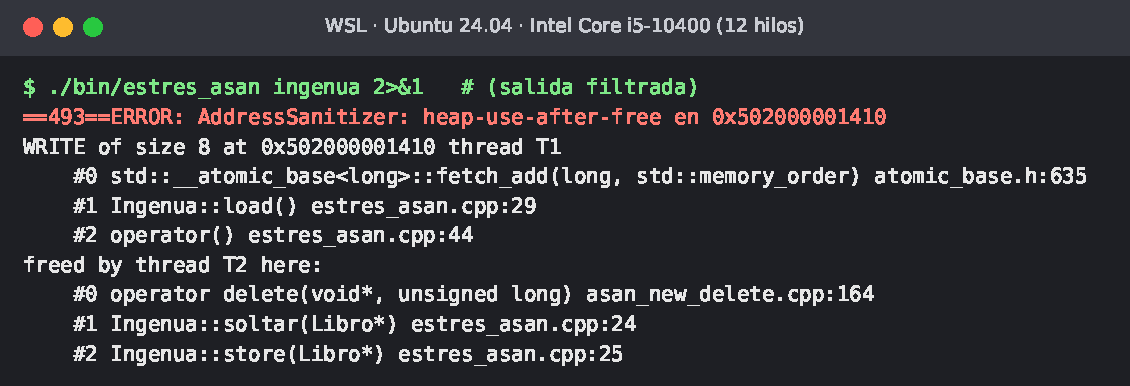
\includegraphics[width=0.98\linewidth,height=0.5\textheight,keepaspectratio]{graficos/captura_asan_ingenua.pdf}\par\smallskip
  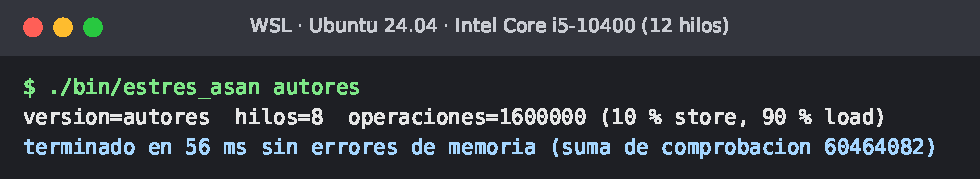
\includegraphics[width=0.7\linewidth,height=0.17\textheight,keepaspectratio]{graficos/captura_asan_autores.pdf}
  \fuente{8 hilos, 10 \% store / 90 \% load en la misma celda. Arriba: versión ingenua. Abajo: código de los autores.}
\end{frame}

\begin{frame}{La idea, antes de pasar a Jheremy}
  \centering
  \begin{tikzpicture}[caja/.style={draw,thick,rounded corners=4pt,align=center,inner sep=7pt}]
    \node[caja,draw=acento,fill=acento!8] (c) {\textbf{Cartel}\\ libro A · talonario \textbf{104}};
    \node[caja,draw=hoja,fill=hoja!8,right=3.2cm of c] (l) {\textbf{Libro A}\\ hoja = \textbf{106} = 104 + 1 + 1};
    \draw[-Latex,thick] (c) -- (l);
    \node[caja,draw=gris,below=1.1cm of c,font=\small] (ana) {pase de Ana (1)};
    \node[caja,draw=gris,right=0.4cm of ana,font=\small] (beto) {pase de Beto (1)};
    \draw[-Latex,gris] (ana) -- (l); \draw[-Latex,gris] (beto) -- (l);
  \end{tikzpicture}
  \bigskip
  \begin{itemize}
    \item Los tickets del talonario \textbf{ya están apuntados} en la hoja del libro: son referencias pagadas por adelantado.
    \item Leer = \clave{arrancar un ticket} con un \texttt{fetch\_and\_add}, que a la vez dice qué libro hay. La hoja no se toca.
    \item Leer y apuntarse pasan a ser \textbf{un solo paso}: la ventana peligrosa desaparece.
  \end{itemize}
\end{frame}

\expone{Jheremy}

\begin{frame}{Conteo de referencias ponderado (Bevan; Watson y Watson, 1987)}
  \begin{columns}[T]
    \column{0.47\textwidth}
    \begin{itemize}\small
      \item Cada referencia tiene un \textbf{peso}; el contador es la \textbf{suma de pesos}.
      \item Soltar: restar su peso.
      \item \textbf{Clonar}: repartir el peso, \clave{sin tocar el contador}.
      \item Clonar una de peso 1 exige subir antes su peso.
    \end{itemize}
    \column{0.5\textwidth}
    \renewcommand{\arraystretch}{1.2}\small
    \begin{tabular}{@{}llcc@{}}
      \toprule
      Acción & Pesos & Hoja & ¿Toca la hoja?\\
      \midrule
      inicio & X = 10 & 10 & ---\\
      clonar X en Y & X = 6, Y = 4 & 10 & \textbf{no}\\
      tirar Y & X = 6 & 6 & sí ($-4$)\\
      clonar X en Z & X = 3, Z = 3 & 6 & \textbf{no}\\
      tirar Z y X & --- & 0 & libera\\
      \bottomrule
    \end{tabular}
    \par\medskip
    En memoria compartida, «tocar la hoja» es tocar una posición lejana: evitarlo es lo que \clave{elimina la carrera}.
  \end{columns}
\end{frame}

\begin{frame}{El peso en el \emph{atomic shared pointer}}
  \begin{columns}[c]
    \column{0.55\textwidth}
    \includegraphics[width=\linewidth]{figuras/paper_fig2.pdf}
    \fuente{Fig. 2 del paper. (a) 104 + 1 + 1 = 106. (b) Tras un \texttt{load}: cartel 103, un pase nuevo, hoja sigue en 106.}
    \column{0.42\textwidth}\footnotesize
    \begin{itemize}
      \item Al crear el cartel se le da un peso $C \gg P$ y se suma $C$ a la hoja. Cada pase pesa 1.
      \item Invariante: \textbf{hoja $\ge$ peso del cartel + pases}. Por arriba es seguro; por abajo, liberaríamos con lectores dentro.
    \end{itemize}
  \end{columns}
  \medskip
  \begin{itemize}\footnotesize
    \item \textbf{Empaquetado}: el peso va en los 16 bits altos libres del puntero (x86-64 usa 48). Restar un ticket es restar $2^{48}$ a la palabra entera; la dirección no cambia:
  \end{itemize}
  \centering{\ttfamily\footnotesize 0x\textcolor{acento}{0068}\,7F3A12345670 $-$ 0x\textcolor{acento}{0001}\,000000000000 = 0x\textcolor{acento}{0067}\,7F3A12345670}
\end{frame}

\begin{frame}{Algoritmo 1: \texttt{store} y \texttt{load}}
  \centering\includegraphics[width=0.7\linewidth]{figuras/paper_alg1.pdf}
  \fuente{Algoritmo 1 del paper.}
  \begin{columns}[T]
    \column{0.48\textwidth}\footnotesize
    \textbf{\texttt{store}}: \textbf{1.} sumar $C$ al objeto nuevo \emph{antes} de publicarlo; \textbf{2.} \texttt{swap}: poner (nuevo, $C$) y llevarse (viejo, $w$) de golpe; \textbf{3.} restar al viejo \textbf{solo} el sobrante $w$.
    \column{0.48\textwidth}\footnotesize
    \textbf{\texttt{load}}: \textbf{1.} \texttt{fetch\_and\_add}($-$\texttt{pack(null,1)}): un ticket menos y el valor anterior: \clave{una instrucción}; \textbf{2.} si quedan menos de $P$: recargar (alg.\,2); \textbf{3.} devolver un pase de peso 1.
  \end{columns}
\end{frame}

\begin{frame}{Por qué desaparece la carrera}
  {\small Cartel (A, 5), hoja de A = 5. Ana: \texttt{load} = un \texttt{fetch\_and\_add} (F). Beto: \texttt{store(B)} = sumar $C$ a B (S1), \texttt{swap} (S2), restar sobrante a A (S3). F y S2 tocan \textbf{la misma palabra}: el procesador los ordena.}
  \medskip
  \begin{columns}[T]
    \column{0.48\textwidth}
    \begin{block}{Caso 1: F antes que S2}
      \small Ana arranca un ticket: cartel (A, 4), Ana tiene un pase de A.\\
      S2 recoge (A, 4); S3 resta 4: hoja de A = 5 $-$ 4 = \textbf{1} = el pase de Ana.\\
      A vive mientras Ana lo usa y se libera cuando lo suelta.
    \end{block}
    \column{0.48\textwidth}
    \begin{block}{Caso 2: F después de S2}
      \small El cartel ya muestra (B, $C$): Ana se lleva un pase de \textbf{B}, respaldado desde S1.\\
      S3 resta 5 a A: se libera sin nadie dentro.\\
      Ana nunca toca A.
    \end{block}
  \end{columns}
  \bigskip
  \centering\clave{No hay tercer caso}: el estado «he leído pero no me he apuntado» ya no existe.
\end{frame}

\begin{frame}{Recargar el talonario: el punto delicado}
  \begin{columns}[T]
    \column{0.52\textwidth}\small
    Cuando un \texttt{load} deja el peso por debajo de $P$, \textbf{ese hilo} recarga: reserva $C-w$ en la hoja y sube el peso lo mismo. Hace falta un \textbf{CAS} («solo si sigue como lo vi»): el cartel pudo cambiar de libro u otro hilo pudo recargar ya.
    \begin{block}{Requisitos para ser \emph{wait-free}}
      \footnotesize\textbf{R-1}: $C \ge 2P$ (tras recargar, el peso queda $\ge 2P-(P-1) = P+1$).\\
      \textbf{R-2}: el peso solo \textbf{baja de 1 en 1} o se \textbf{fija por encima de $P$}.
    \end{block}
    \column{0.44\textwidth}
    \includegraphics[width=\linewidth]{figuras/paper_fig4.pdf}
    \fuente{Fig. 4 del paper: peso de un cartel en el tiempo; la línea es $P$.}
  \end{columns}
  \medskip\small
  Si el CAS falla y el peso \textbf{subió}, alguien ya recargó: \clave{salida temprana}. Quien mete el talonario en la zona roja, lo saca; si otro se adelanta, se va.
\end{frame}

\begin{frame}{Algoritmo 2: \texttt{increase\_weight}}
  \centering\includegraphics[width=0.7\linewidth]{figuras/paper_alg2.pdf}
  \fuente{Algoritmo 2 del paper.}
  \begin{columns}[T]
    \column{0.55\textwidth}\footnotesize
    \textbf{1.} reservar $C-w$ en la hoja \textbf{antes} del CAS; \textbf{2.} CAS: si el cartel sigue en (ptr, actual), sumar $C-w$ y terminar; \textbf{3.} otro puntero o \textbf{peso mayor}: devolver la reserva y salir; \textbf{4.} peso menor: reintentar.
    \column{0.41\textwidth}\footnotesize
    Los pesos esperados forman una cadena \textbf{estrictamente decreciente} entre $P-1$ y 0: \clave{como mucho $P$ intentos}.
  \end{columns}
\end{frame}

\begin{frame}{Demo 2: un simulador encuentra los fallos de cada variante}
  \centering
  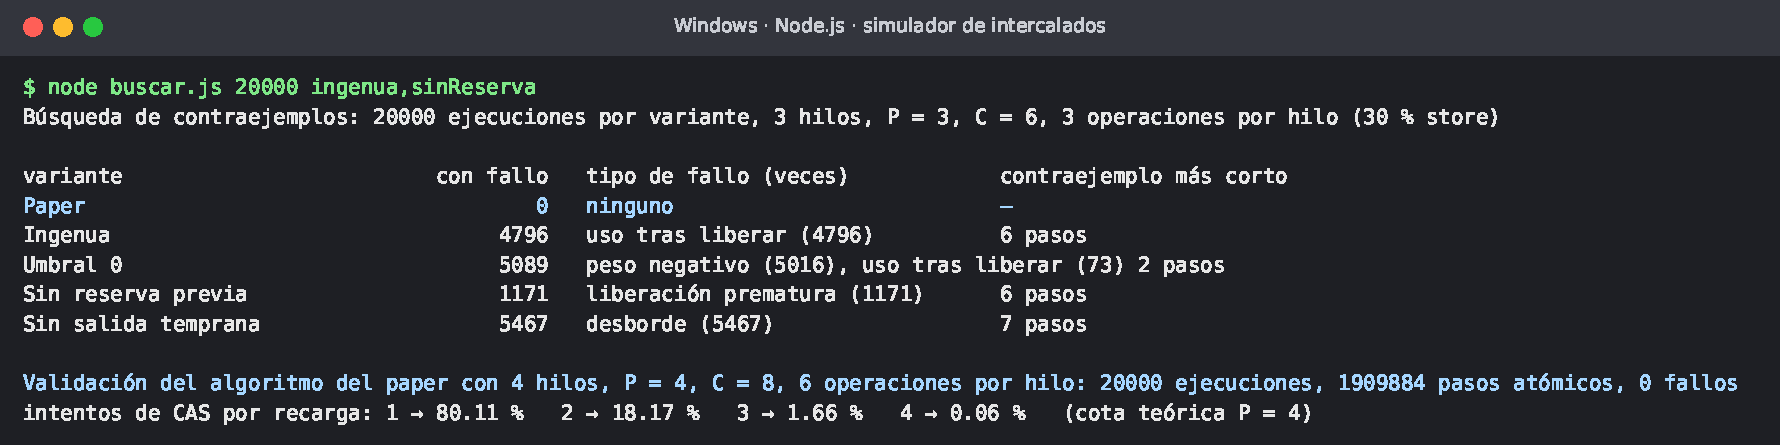
\includegraphics[width=0.98\linewidth]{graficos/captura_simulador.pdf}
  \begin{itemize}\footnotesize\raggedright
    \item Simulador de intercalados (paso atómico a paso atómico) que comprueba los invariantes tras cada paso, 20\,000 ejecuciones por variante. \textbf{Paper: 0 fallos}; cada variante rota falla en 2 a 7 pasos.
    \item Ejemplo («sin reserva»): Carla hace \texttt{load} y le toca recargar; Beto hace \texttt{swap} y resta toda la reserva: el libro se libera \textbf{con un lector dentro}.
  \end{itemize}
\end{frame}

\expone{Diego}

\begin{frame}{La demostración: el peso nunca es negativo}
  \begin{columns}[T]
    \column{0.5\textwidth}
    \small
    \textbf{Por qué importa}: el peso está en 16 bits sin signo; $-1$ sería 65\,535 \emph{tickets fantasma} sin respaldo $\Rightarrow$ \emph{use-after-free}.\par\medskip
    \textbf{Ofensa}: decrementar el peso cuando vale $\le P$.\\
    \textbf{$O$}: multiconjunto de ofensores; se vacía cuando alguien fija el peso por encima de $P$.
    \column{0.47\textwidth}
    \small
    \textbf{Invariante 1}: cada hilo está en $O$ como mucho una vez (quien ofende recarga, y no sale sin que $O$ se vacíe).\par\medskip
    \textbf{Invariante 2}: peso $\ge P - |O|$ (desde el último vaciado solo baja de 1 en 1; cada bajada en zona roja suma 1 a $|O|$).
  \end{columns}
  \bigskip
  \begin{block}{}
    \centering\large peso $\ \ge\ P - |O|\ \ge\ P - P\ =\ 0$
  \end{block}
  \small Por eso el umbral de recarga es $P$ y no 0: es el colchón para que todos ofendan una vez a la vez.
\end{frame}

\begin{frame}{Coste y extensiones}
  \begin{columns}[T]
    \column{0.52\textwidth}\footnotesize
    \begin{itemize}
      \item El bucle CAS solo repite si \textbf{otro} hilo bajó el peso: cadena $w_0 > w_1 > \dots \ge 0$ con $w_0 \le P-1$ $\Rightarrow$ como mucho $P$ intentos.
      \item \texttt{load}: normalmente una instrucción; \textbf{$O(P)$ solo en el peor caso} ($P$ = hilos que usan esa variable). Con $C = 2^{19}$, $P = 2^{16}$ hay $\approx$ 458\,752 lecturas entre recargas.
      \item Extensiones: \texttt{null} (el peso da la vuelta, sin recargar), punteros débiles (misma técnica) y \emph{aliasing} (dos punteros en 128 bits).
    \end{itemize}
    \column{0.44\textwidth}
    \renewcommand{\arraystretch}{1.15}\footnotesize
    \begin{tabular}{@{}p{2.1cm}p{1.9cm}l@{}}
      \toprule
      Operación & Coste & Garantía\\
      \midrule
      \texttt{store}, \texttt{swap} & $O(1)$ & \emph{wait-free}\\
      \texttt{load} & 1 instr.; $O(P)$ peor & \emph{wait-free}\\
      compare-and-swap & sin cota & \emph{lock-free}\\
      \texttt{load} \emph{aliased} & sin cota & \emph{lock-free}\\
      \bottomrule
    \end{tabular}
    \par\smallskip{\scriptsize El CAS es \emph{lock-free}: cualquier lectura cambia los tickets y hace fallar al escritor.}
  \end{columns}
\end{frame}

\begin{frame}{Experimentos del paper}
  \begin{columns}[c]
    \column{0.5\textwidth}\footnotesize
    \begin{itemize}
      \item $C = 2^{19}$, $P = 2^{16}$. Rendimiento: 144 hilos; latencia: 56 hilos.
      \item Banco: \textbf{pila concurrente} ($n$ pilas, $u$\,\% de actualizaciones). Rivales: Libstdc++ (candados), Williams y Folly (\emph{split refcount}), Anderson (\emph{hazard pointers}).
      \item Con 1 hilo, \textbf{Ours} es la más rápida; gana a los que no usan memoria extra (con 1 pila y 144 hilos, $\approx$7× Williams y $\approx$20× Folly). Frente a Anderson depende de la contención: pierde con una sola pila.
      \item \texttt{load}, $p = 56$ (mediana): \textbf{Ours 1,14\us} · Anderson 2,58\us · Folly 11,6\us · Libstdc++ 99,7\us.
    \end{itemize}
    \column{0.46\textwidth}
    \includegraphics[width=\linewidth]{figuras/paper_fig5.pdf}
    \fuente{Fig. 5 del paper: millones de operaciones por segundo frente a hilos.}
  \end{columns}
\end{frame}

\begin{frame}{Pruebas en local (1): el boceto y sus variantes rotas}
  \centering
  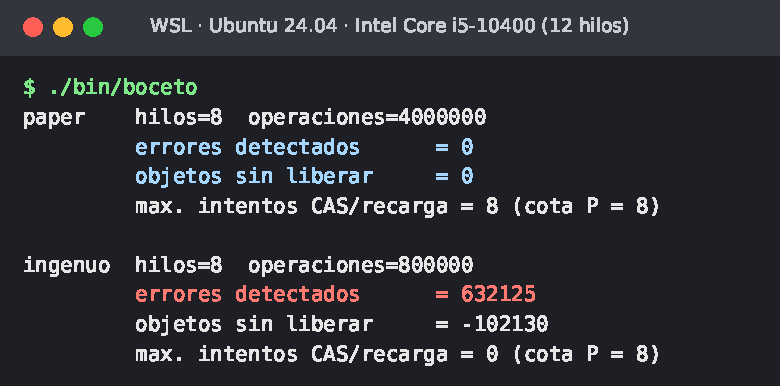
\includegraphics[width=0.8\linewidth,height=0.22\textheight,keepaspectratio]{graficos/captura_boceto.pdf}\par\smallskip
  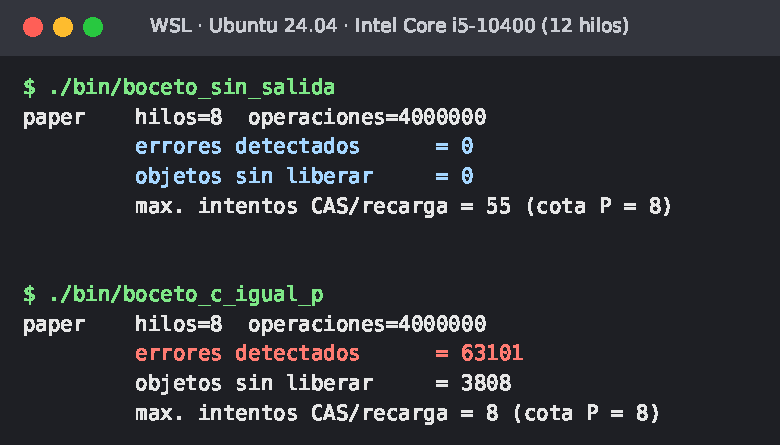
\includegraphics[width=0.98\linewidth,height=0.36\textheight,keepaspectratio]{graficos/captura_boceto_variantes.pdf}
  \begin{itemize}\footnotesize
    \item Boceto en C++, $P = 8$, $C = 16$. Paper: \textbf{0 errores}, como mucho 7 intentos ($\le P$). Ingenua: 601\,681 errores y dobles liberaciones.
    \item Sin salida temprana: 0 errores pero \textbf{38 intentos} $> P$ (no \emph{wait-free}). Con $C = P$ (rompe R-1): 50\,060 errores.
  \end{itemize}
\end{frame}

\begin{frame}{Pruebas en local (2): rendimiento con el código de los autores}
  \centering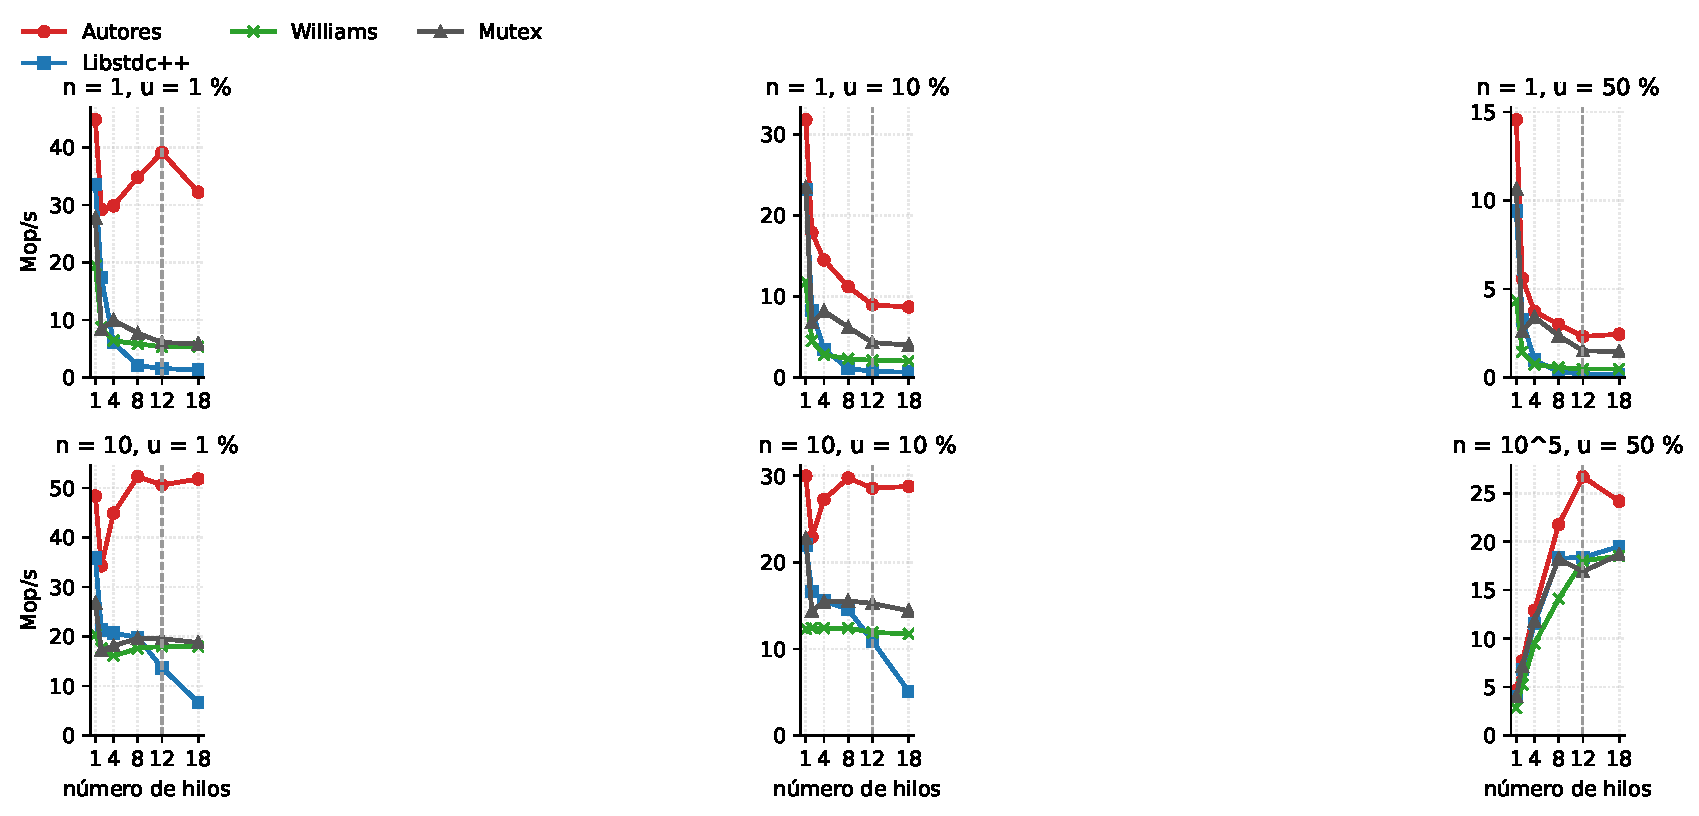
\includegraphics[width=0.74\linewidth]{graficos/local_rendimiento.pdf}
  \fuente{Mini-Fig. 5 (12 hilos): Autores, \texttt{atomic<shared\_ptr>} de GCC 13 (Libstdc++) y \texttt{std::mutex}. $n=1,u=1$: 34,3 · 2,2 · 6,4 Mop/s. Con $n=1,u=50$ el mutex gana (2,9 frente a 2,2): el CAS es \emph{lock-free}. Con 1 hilo, Autores es la más rápida. Tendencias, no cifras absolutas.}
\end{frame}

\begin{frame}{Pruebas en local (3): latencia con 12 hilos}
  \centering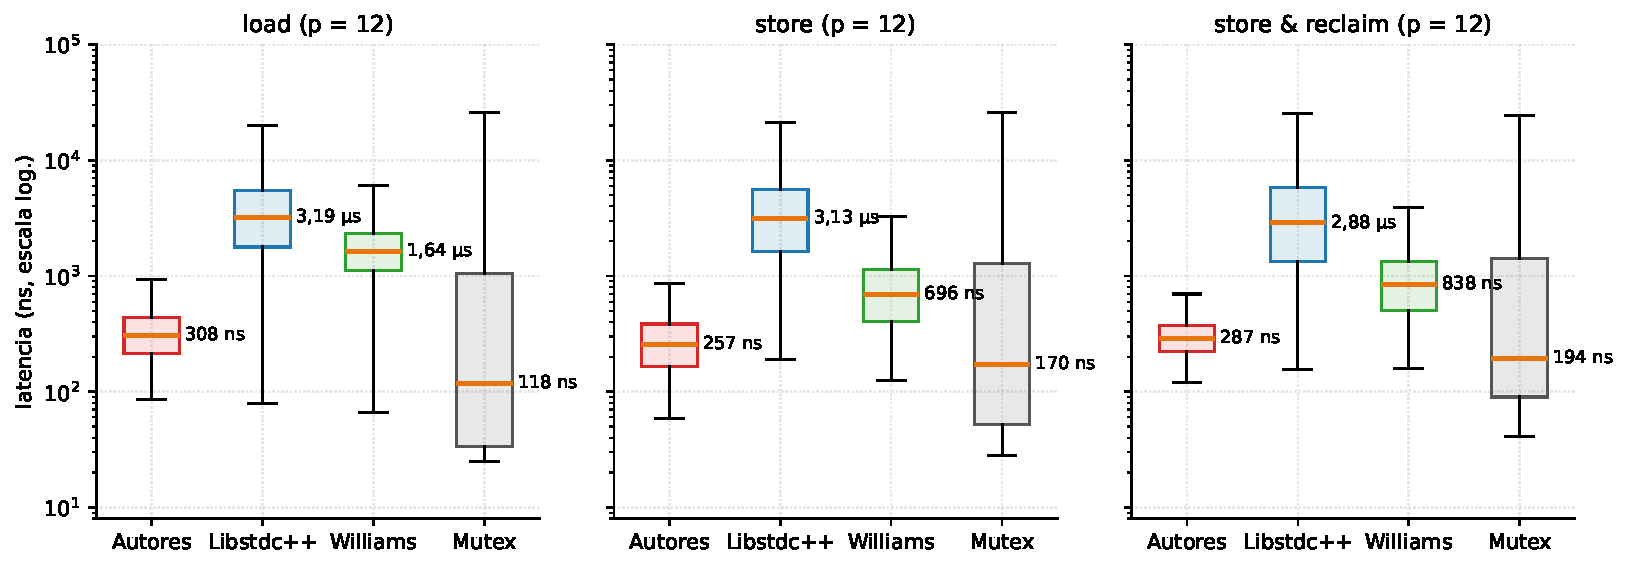
\includegraphics[width=0.72\linewidth]{graficos/local_latencia.pdf}
  \fuente{Mini-Fig. 6: 1 hilo mide y 11 hacen \texttt{store}; 100\,000 muestras. \texttt{load} (mediana / p99): Autores 269 ns / 0,83\us · Libstdc++ 3,06\us{} / 16\us · Mutex 61 ns / \textbf{27,6\us}. La mediana engaña; la cola delata a quien espera.}
\end{frame}

\begin{frame}{Valoración crítica}
  \begin{columns}[T]
    \column{0.48\textwidth}
    \textbf{\textcolor{ok}{Fortalezas}}
    \begin{itemize}\small
      \item Sencillo: unas 30 líneas de núcleo y una demostración de una página.
      \item \texttt{load}/\texttt{store}/\texttt{swap} \emph{wait-free}, sin memoria extra, liberación inmediata (rc = 1 fiable).
      \item Lecturas de una instrucción: menor latencia y cola corta.
      \item Mejora software real (Folly, GCC) y publica su código.
    \end{itemize}
    \column{0.48\textwidth}
    \textbf{\textcolor{mal}{Límites}}
    \begin{itemize}\small
      \item CAS y \emph{aliasing} solo \emph{lock-free}.
      \item Cada lectura \textbf{escribe} en la variable compartida (no hay \emph{snapshot pointers}).
      \item Límite estricto de $P$ hilos: es de \textbf{corrección}, no de rendimiento.
      \item Depende de bits libres en el puntero (paginación de 5 niveles, ARM con PAC/MTE).
      \item No discute el orden de memoria; evalúa una estructura y una arquitectura.
    \end{itemize}
  \end{columns}
\end{frame}

\begin{frame}{Conclusiones}
  \begin{enumerate}\small
    \item El conteo de referencias con variables mutables puede ser \clave{wait-free sin retrasar la liberación}.
    \item La clave: un \textbf{peso prepagado} en el propio puntero; leer y apuntarse son una sola instrucción.
    \item La recarga termina en como mucho $P$ intentos gracias a R-1 ($C \ge 2P$) y R-2 (salida temprana).
    \item Funciona en la práctica: lo comprobamos en local con el código original (sin errores y mucho más rápido que la versión con candados bajo contención).
  \end{enumerate}
  \bigskip
  \textbf{Para discutir}
  \begin{itemize}\small
    \item ¿Se podría hacer el compare-and-swap \emph{wait-free} (técnicas de ayuda entre hilos) sin perder rapidez?
    \item ¿Compensaría un modo de lectura sin escritura para variables que casi nunca cambian?
  \end{itemize}
\end{frame}

{\setbeamertemplate{footline}{}
\begin{frame}[plain]
  \centering\vfill
  {\fontsize{32}{36}\selectfont\bfseries ¿Preguntas?}\par\bigskip
  {\large David · Jheremy · Diego}\par\vfill
  {\small\color{gris}Código, capturas y gráficas de esta exposición: carpeta \texttt{exposicion\_paper/} (\texttt{codigo/ejecutar\_pruebas.sh})}
  \vspace*{6mm}
\end{frame}}

\expone{}

\begin{frame}{Referencias}
  \scriptsize
  \begin{itemize}
    \item I. G. de Wolff, D. Anderson, G. K. Keller y A. Seletskiy. \emph{A Fast Wait-Free Solution to Read-Reclaim Races in Reference Counting}. Euro-Par 2024, LNCS 14803, págs. 103–118. Springer. doi:10.1007/978-3-031-69583-4\_8.
    \item Código de los autores: \texttt{github.com/ivogabe/wait-free-atomic-shared-pointer} (commit 8540c58); artefacto en Zenodo, doi:10.5281/zenodo.11775182.
    \item M. Herlihy. Wait-free synchronization. \emph{ACM TOPLAS} 13(1), 1991.
    \item D. I. Bevan; P. Watson e I. Watson. Conteo de referencias ponderado. PARLE 1987.
    \item D. Detlefs, P. Martin, M. Moir y G. Steele. Lock-free reference counting. PODC 2001.
    \item H. Sundell. Wait-free reference counting and memory management. IPDPS 2005.
    \item D. Anderson, G. Blelloch e Y. Wei. Concurrent deferred reference counting with constant-time overhead. PLDI 2021.
    \item A. Williams. \emph{C++ Concurrency in Action}. Manning, 2012.
    \item Artefacto 1: \url{https://claude.ai/artifact/YBS98Wz8SmSYWHca2YbHF6}
    \item Artefacto 2: \url{https://claude.ai/artifact/EQJd2aXZUYVX1Zio4DqFwH}
    \item Artefacto 3: \url{https://claude.ai/artifact/VVGviffH178bBZ6tGSAnKZ}
  \end{itemize}
  \fuente{Figuras y algoritmos «del paper»: reproducidos de la publicación original con fines académicos.}
\end{frame}

\end{document}
